% 2137 Lab 1 Report
% Created: 2020-01-16, Xingpeng Yi

%==========================================================
%=========== Document Setup  ==============================

% Formatting defined by class file
\documentclass[11pt]{article}

% ---- Document formatting ----
\usepackage[margin=1in]{geometry}	% Narrower margins
\usepackage{booktabs}				% Nice formatting of tables
\usepackage{graphicx}				% Ability to include graphics

%\setlength\parindent{0pt}	% Do not indent first line of paragraphs 
\usepackage[parfill]{parskip}		% Line space b/w paragraphs
%	parfill option prevents last line of pgrph from being fully justified

% Parskip package adds too much space around titles, fix with this
\RequirePackage{titlesec}
\titlespacing\section{0pt}{8pt plus 4pt minus 2pt}{3pt plus 2pt minus 2pt}
\titlespacing\subsection{0pt}{4pt plus 4pt minus 2pt}{-2pt plus 2pt minus 2pt}
\titlespacing\subsubsection{0pt}{2pt plus 4pt minus 2pt}{-6pt plus 2pt minus 2pt}

% ---- Hyperlinks ----
\usepackage[colorlinks=true,urlcolor=blue]{hyperref}	% For URL's. Automatically links internal references.

% ---- Code listings ----
\usepackage{listings} 					% Nice code layout and inclusion
\usepackage[usenames,dvipsnames]{xcolor}	% Colors (needs to be defined before using colors)

% Define custom colors for listings
\definecolor{listinggray}{gray}{0.98}		% Listings background color
\definecolor{rulegray}{gray}{0.7}			% Listings rule/frame color

% Style for Verilog
\lstdefinestyle{Verilog}{
	language=Verilog,					% Verilog
	backgroundcolor=\color{listinggray},	% light gray background
	rulecolor=\color{blue}, 			% blue frame lines
	frame=tb,							% lines above & below
	linewidth=\columnwidth, 			% set line width
	basicstyle=\small\ttfamily,	% basic font style that is used for the code	
	breaklines=true, 					% allow breaking across columns/pages
	tabsize=3,							% set tab size
	commentstyle=\color{gray},	% comments in italic 
	stringstyle=\upshape,				% strings are printed in normal font
	showspaces=false,					% don't underscore spaces
}

% How to use: \Verilog[listing_options]{file}
\newcommand{\Verilog}[2][]{%
	\lstinputlisting[style=Verilog,#1]{#2}
}




%======================================================
%=========== Body  ====================================
\begin{document}

\title{ELC 2137 Lab \#9: ALU}
\author{Xingpeng Yi}

\maketitle


\section*{Summary}

This lab explain the difference between combinational and regular sequential logic, describe the operation of an SR latch, D latch, D flip-flop, and D register, describe the differences in Verilog procedural blocks for combinational versus sequential logic, and import and modify modules from a previous project and use them  design a modular system. The lab required students to create an ArithmeticLogic Unit (ALU) capable of a few operations. In order to do mathematical operations with the ALU, we need two numbers. One of these will come from the switches. For the other, we will use a use a register to store a number.


\section*{Q\&A}
None.
\section*{Results}


\begin{table*}[ht]\centering
	\caption{\textit{register} expected results table}
	\label{ALU:tbl:register_ERT}\medskip
	\begin{tabular}{l|rrrrrrrrrrr}
		Time (ns): & 0-5 & 5-10 & 10-15 & 15-20 & 20-25 & 25-30 & 30-35 & 35-40 & 40-45 & 45-50 & 50-55 \\
		\midrule
		D (hex) & 0 & 0 & A & A & 3 & 3 & 0 & 0 & 0$\to$6 & 6 & 6 \\
		clk        & 0 & 1 & 0 & 1 & 0 & 1 & 0 & 1 & 0 & 1 & 0 \\
		en  	& 0 & 0 & 1 & 1 & 1$\to$0 & 0$\to$1 & 1$\to$0 & 0 & 0$\to$1 & 1 & 1 \\
		rst 	& 0 & 0$\to$1 & 0 & 0 & 0 & 0 & 0 & 0 & 0 & 0 & 0 \\
		\midrule
		Q (hex) & X & X$\to$0 & 0 & A & A & A & A & A & 6 & 6 & 6 \\
		\bottomrule
	\end{tabular}
\end{table*}

\begin{figure}[ht]\centering
	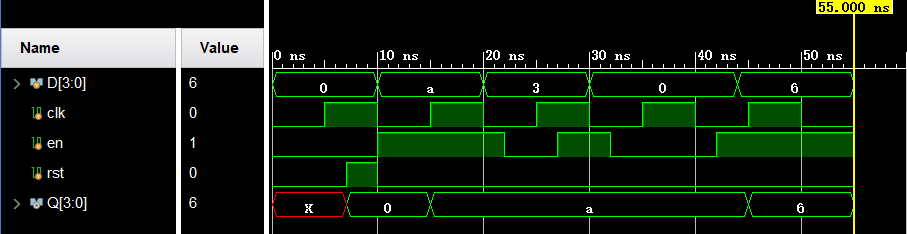
\includegraphics[width=1\textwidth]{register_result.PNG}
	\caption{Register module simulation waveform.}
	\label{fig:register wave}
\end{figure}

\begin{table*}[ht]\centering
	\caption{\textit{alu} expected results table skeleton}
	\label{ALU:tbl:alu_ERT}\medskip
	\begin{tabular}{l|rrrrr}
		Time (ns): & 0-10 & 10-20 & 20-30 & 30-40 & 40-50 \\
		\midrule
		in0 & 00 & 01  & 00 & 00 &  01\\
		in1 & 01 & 00 & 00 & 01 & 01  \\
		op	& 0 & 1 & 2 & 3 & 4 \\
		\midrule
		out & 01 & 01 & 00 & 01 & 00 \\
		\bottomrule
	\end{tabular}
\end{table*}

\begin{figure}[ht]\centering
	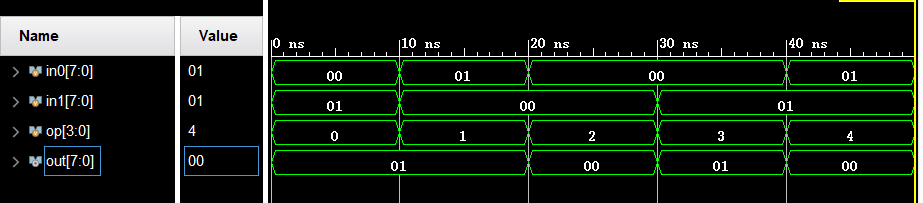
\includegraphics[width=1\textwidth]{alu_result.PNG}
	\caption{ALU module simulation waveform.}
	\label{fig:ALU wave}
\end{figure}

\begin{figure}[ht]\centering
	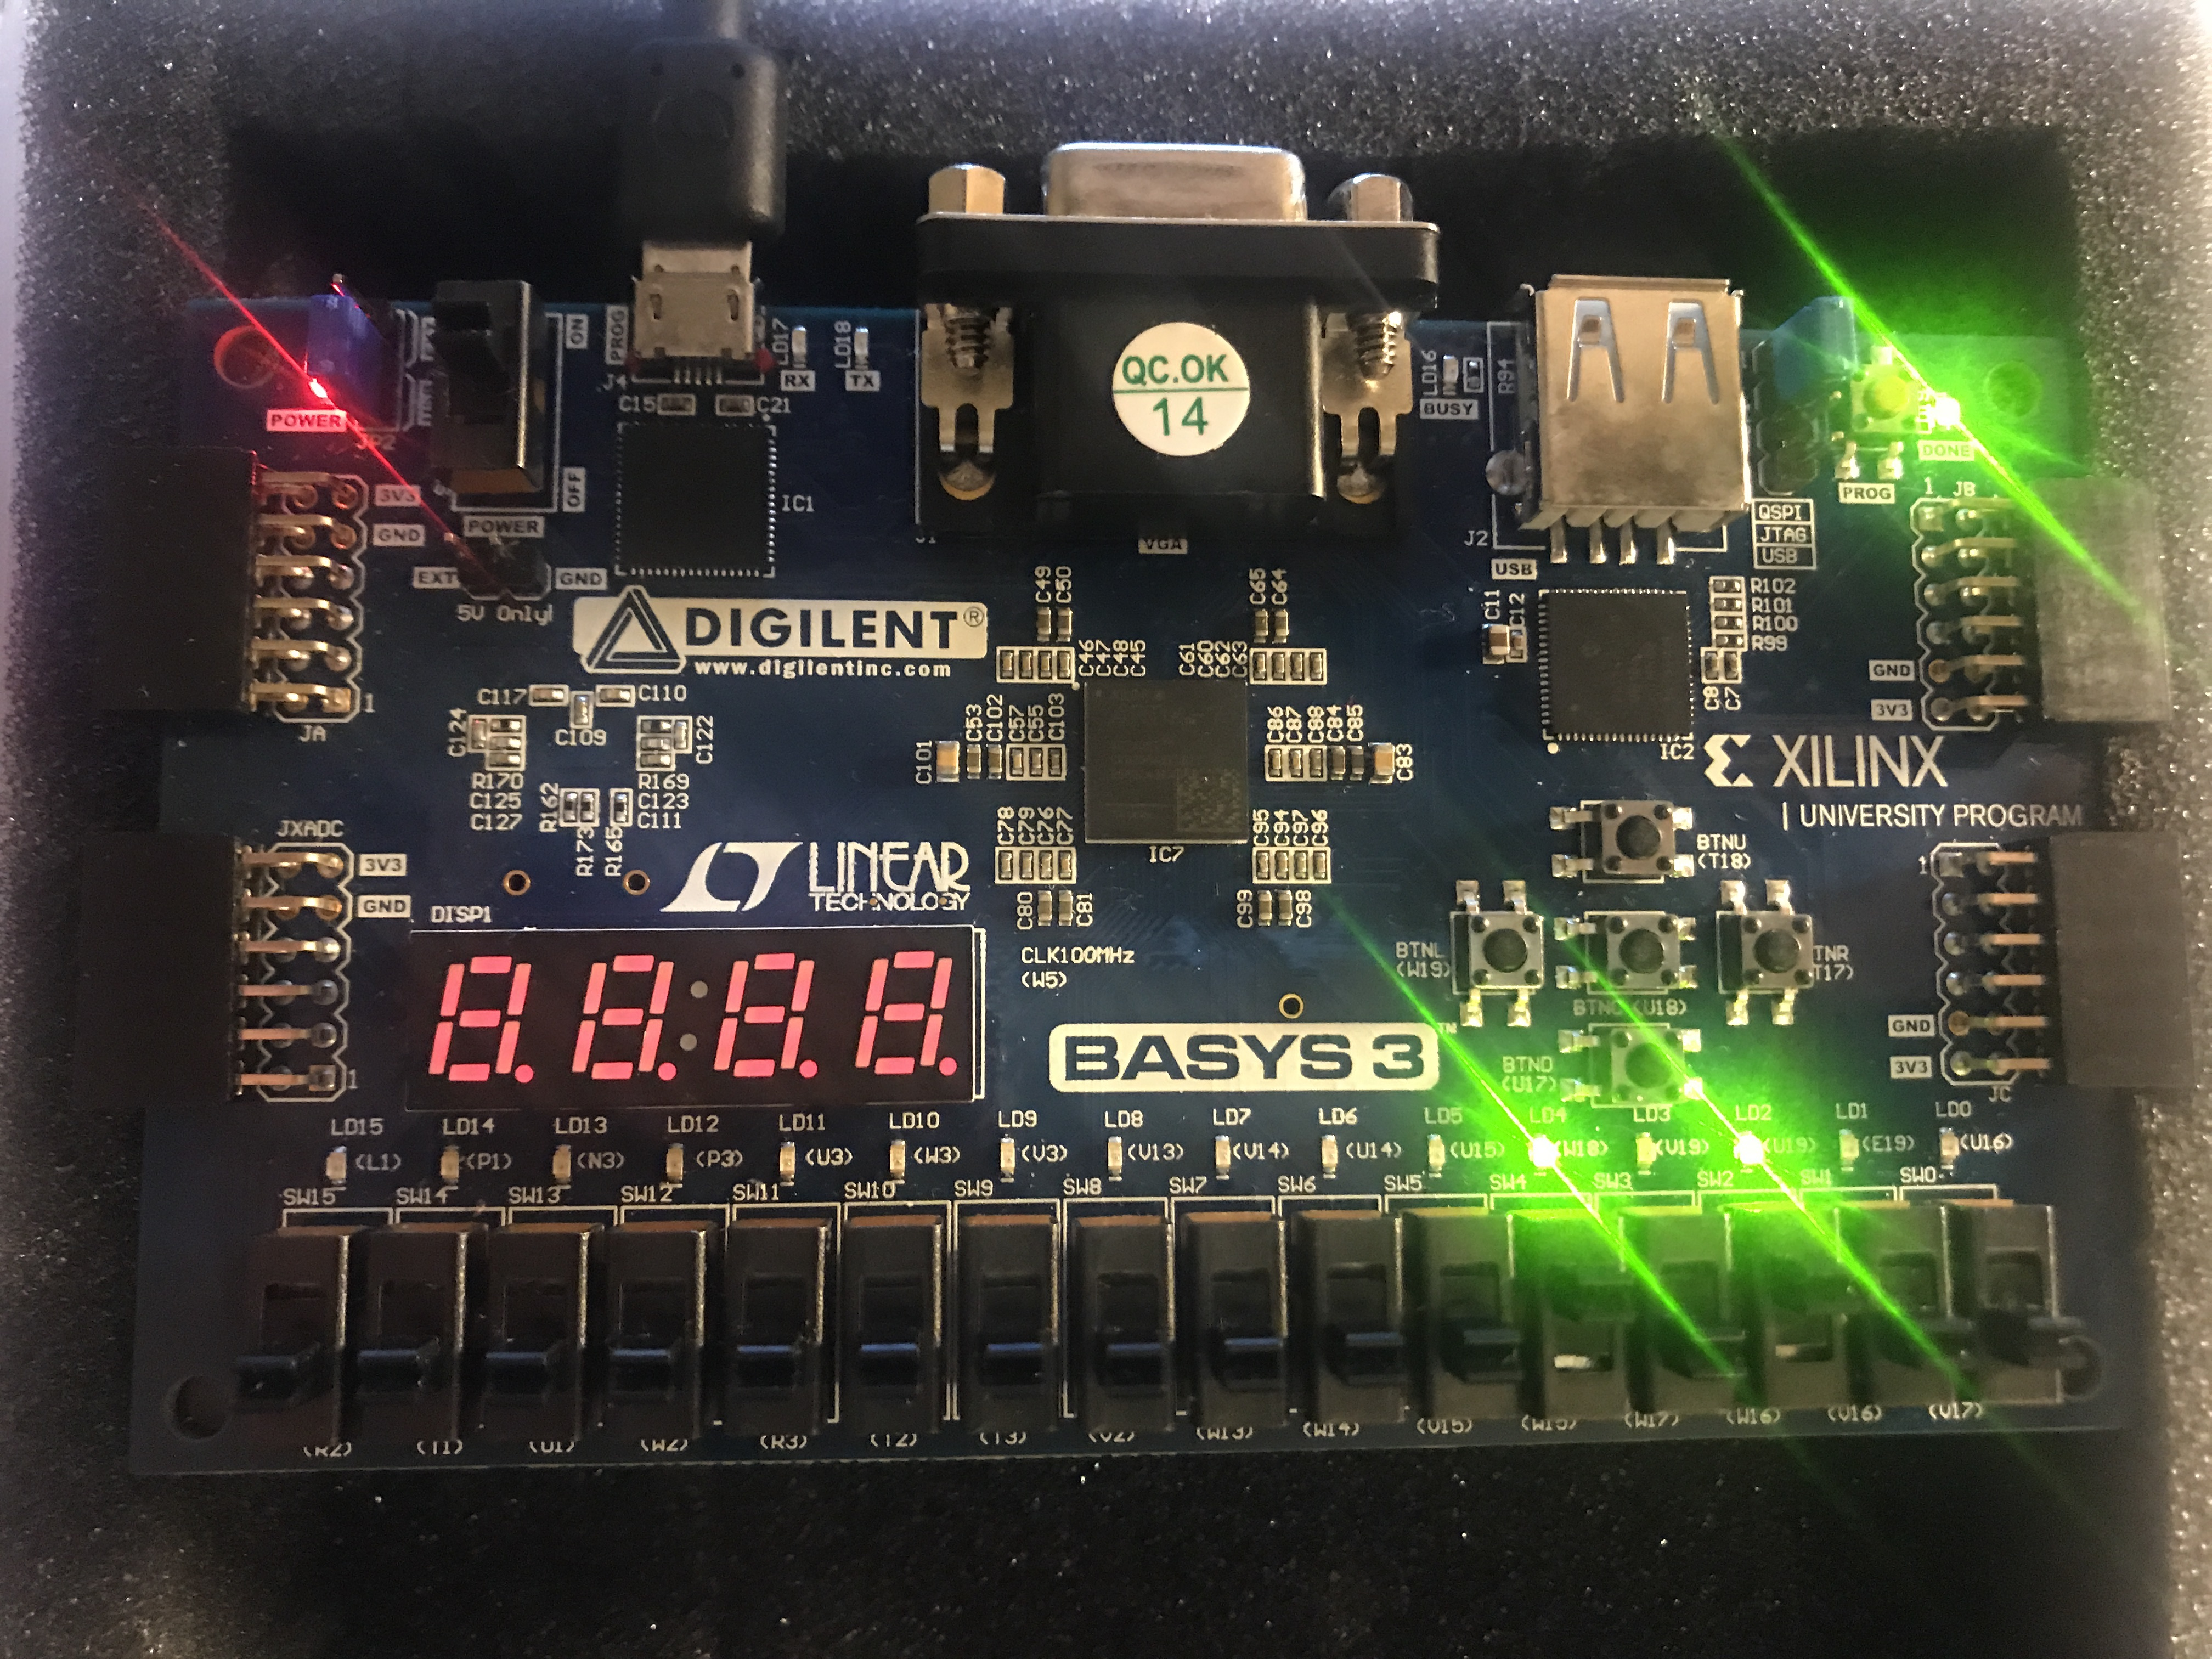
\includegraphics[width=0.5\textwidth]{firststep}
	\caption{Basys 3 board step1.}
	\label{fig:step 1 of board}
\end{figure}

\begin{figure}[ht]\centering
	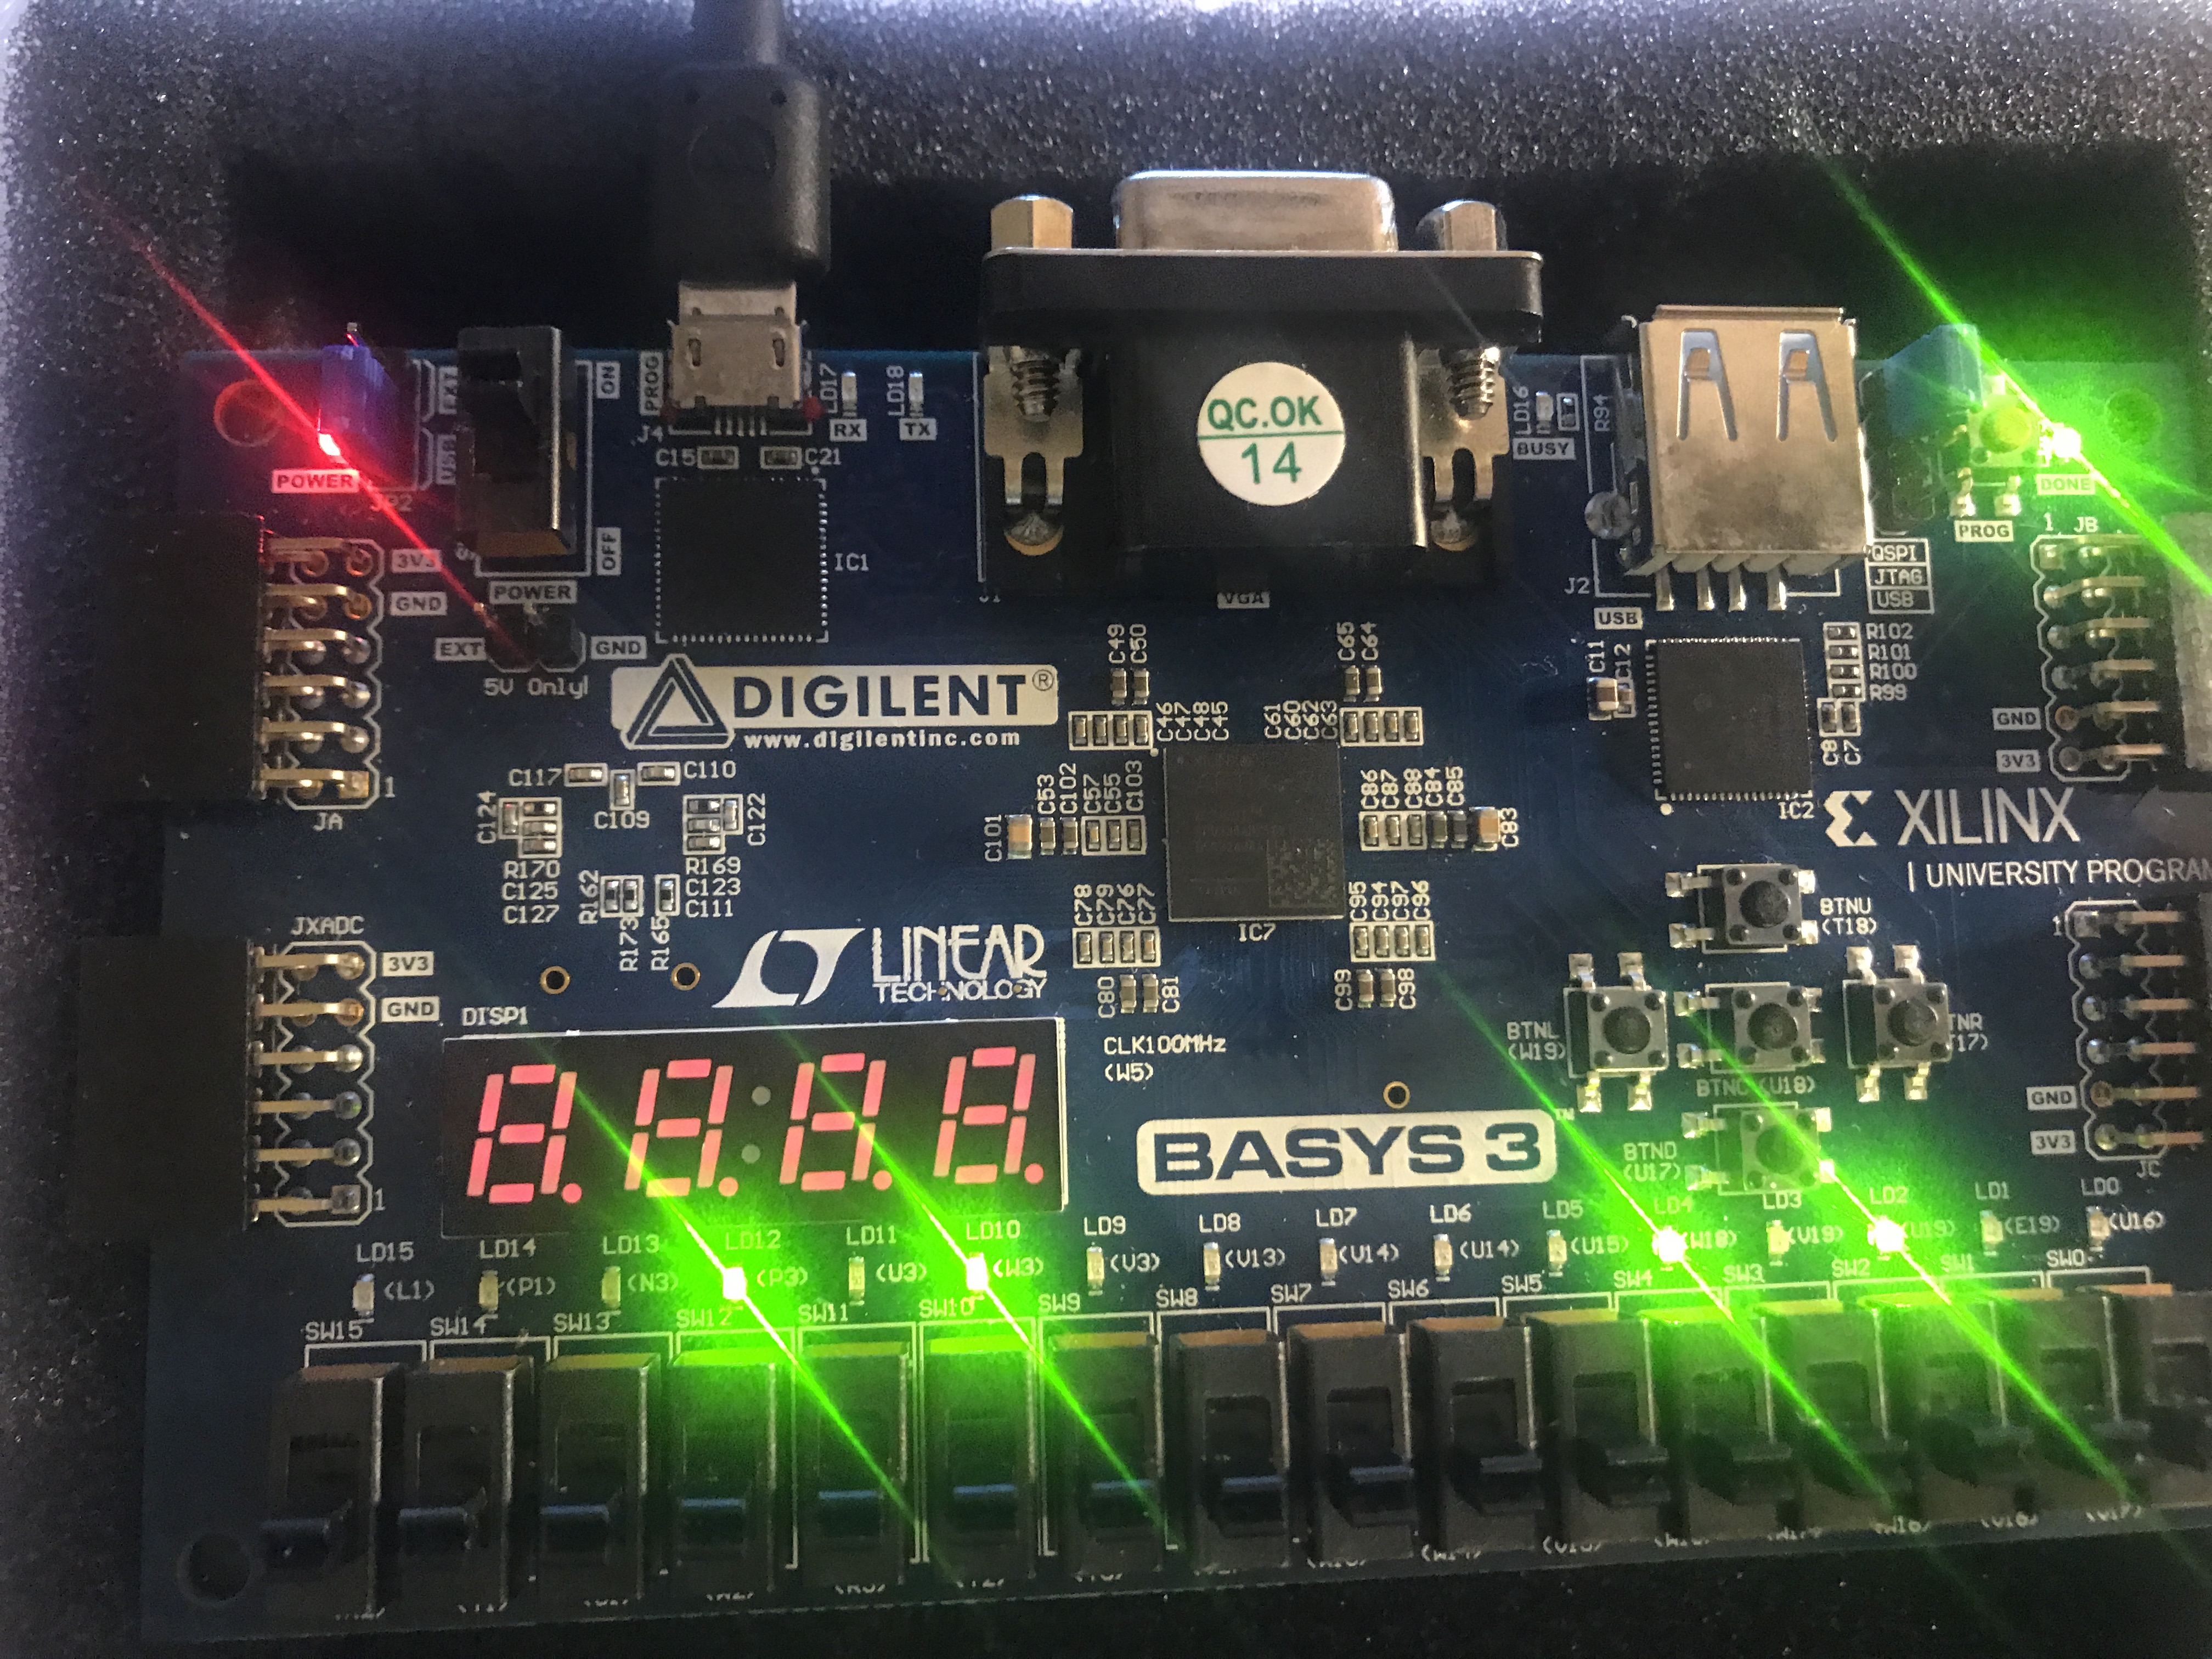
\includegraphics[width=0.5\textwidth]{secondstep}
	\caption{Basys 3 board step2.}
	\label{fig:step 2 of board}
\end{figure}

\begin{figure}[ht]\centering
	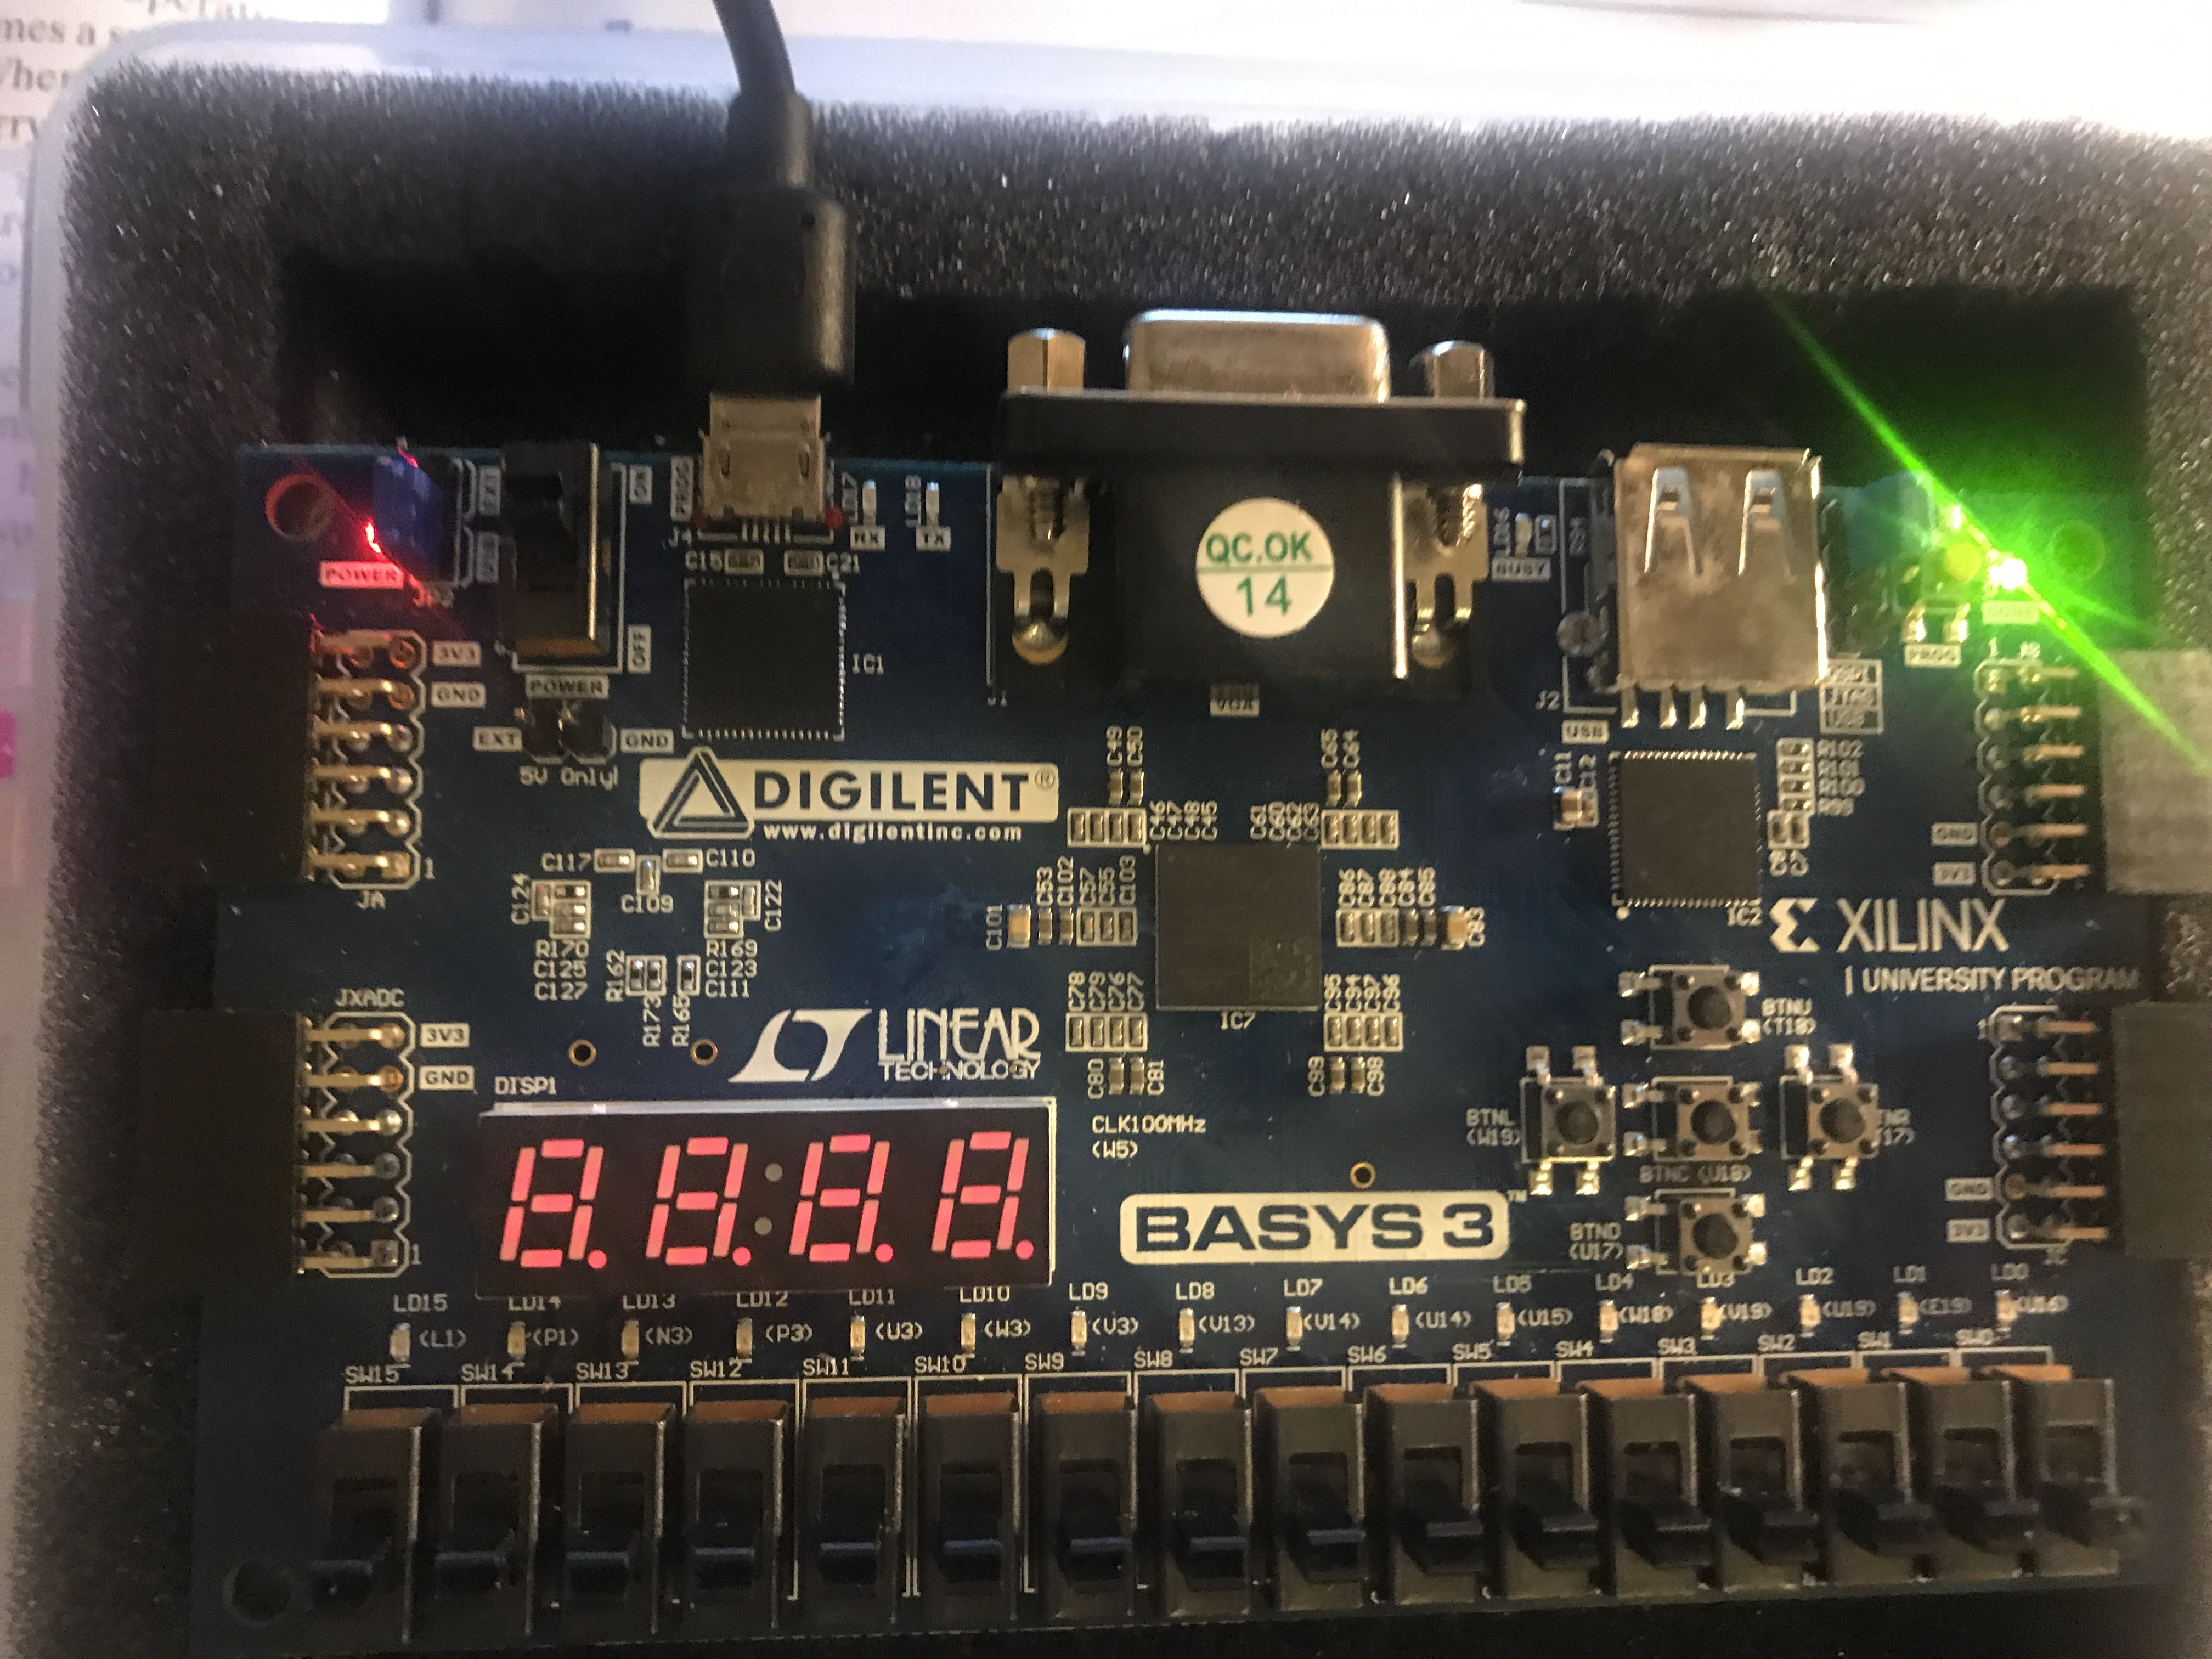
\includegraphics[width=0.5\textwidth]{thirdstep}
	\caption{Basys 3 board step3.}
	\label{fig:step 3 of board}
\end{figure}

\begin{figure}[ht]\centering
	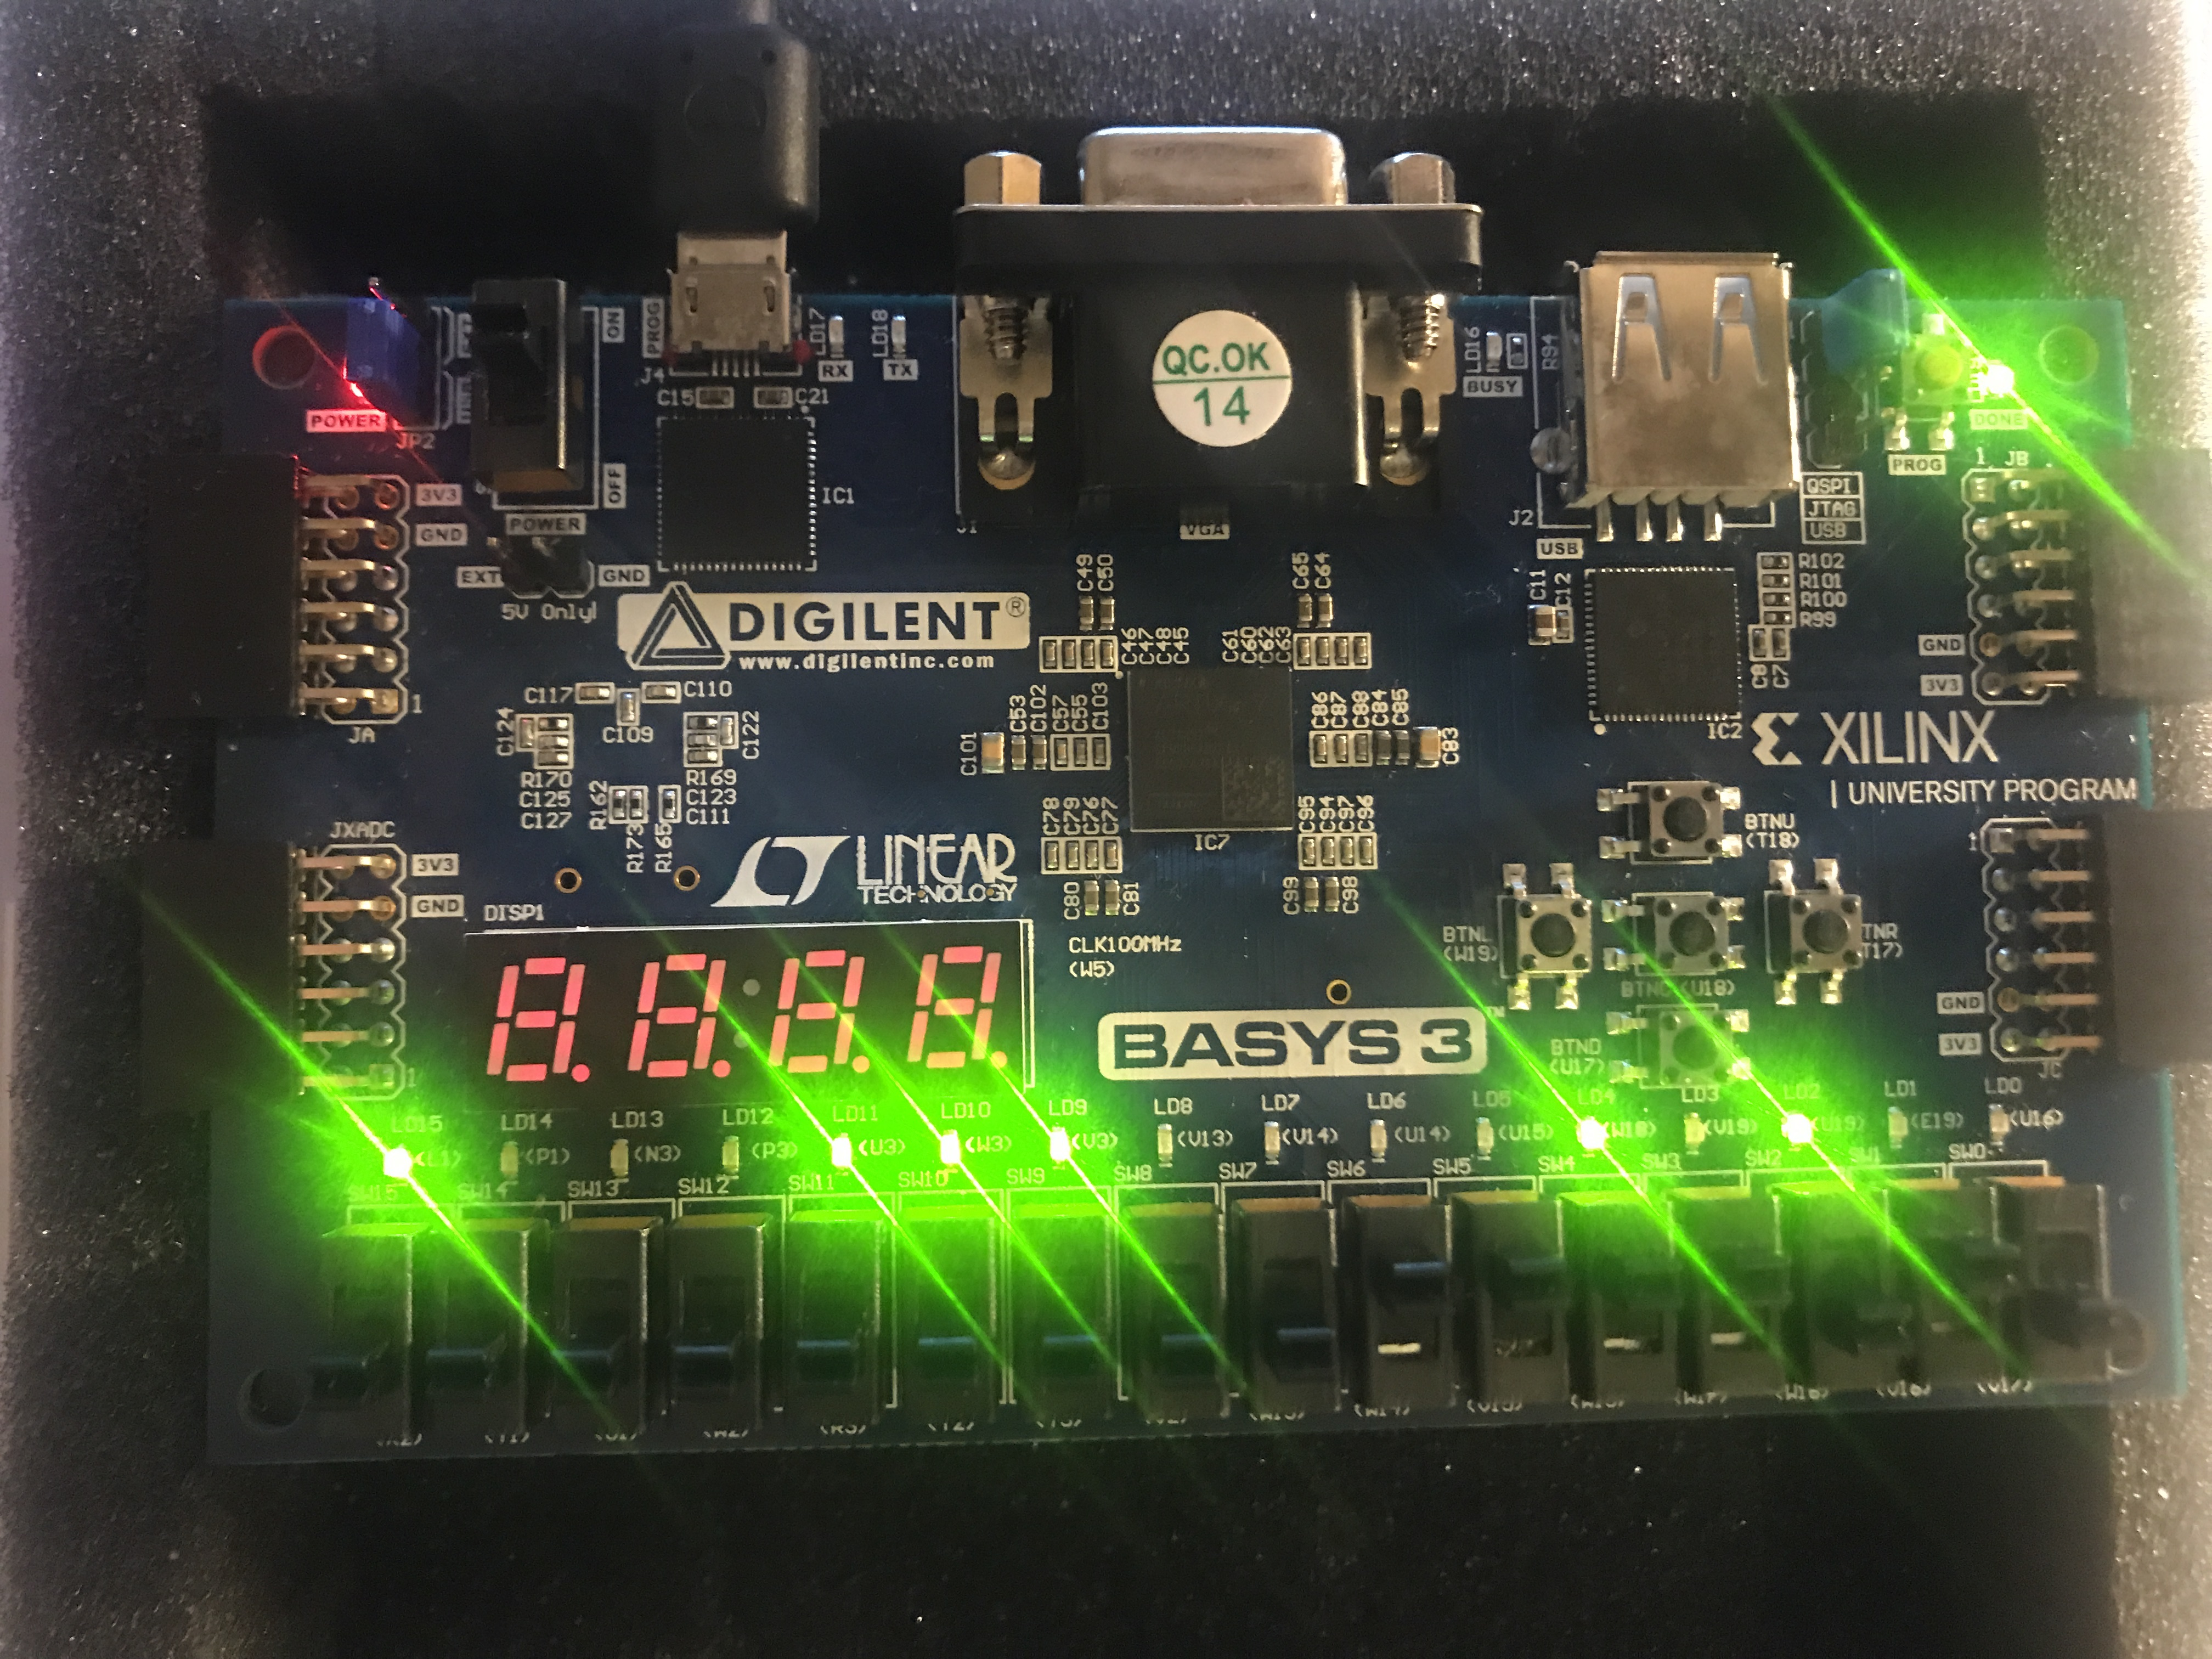
\includegraphics[width=0.5\textwidth]{laststep}
	\caption{Basys board step4.}
	\label{fig:step 4 of board}
\end{figure}

\clearpage
\section*{Code}
\Verilog[firstline=22, lastline=38, caption=register module source file,
label=code:file_ex_lines]{register.sv}

\Verilog[firstline=22, lastline=48, caption=ALU module source file,
label=code:file_ex_lines]{alu.sv}

\Verilog[firstline=22, lastline=40, caption=Top level source file,
label=code:file_ex_lines]{top_lab9.sv}

\Verilog[firstline=22, lastline=48, caption=register module testbench,
label=code:file_ex_lines]{register_test.sv}

\Verilog[firstline=1, lastline=20, caption=ALU module testbench,
label=code:file_ex_lines]{alu_test.sv}




\end{document}
